\documentclass[notes, xcolor=dvipsnames]{beamer}

\usetheme{Warsaw}

\usepackage{inputenc}
\usepackage{amsmath}
\usepackage{graphicx}

\title{Compiler Testing via a Theory of Sound Optimisations in the C11/C++11 Memory Model}
\subtitle{Robin M., Pankaj P., Francesco Z.}

\author{Presented by \\ Akshay Gopalakrishnan}

\begin{document}
    
    \begin{frame}
        
        \maketitle

    \end{frame}

    \begin{frame}{Introduction}

        Testing sequential programs to hunt for compiler bugs is well established at this time. 
        However, testing concurrency bugs still remains a hard problem. 
        This is majorly due to ill understood specification of the memory consistency model, and lack of information on the various transformations that preserve concurrent program semantics.
        This work designs a strategy to reduce the complexity of finding concurrency bugs in C11/C++11 via testing sequential code.
        The source code trace is compared with that of the final end code trace.
        Previous theoretical work establishing soundness of various local transformations in concurrent execution is utilized to achieve this. 
        
    \end{frame}

    \begin{frame}{Example of Compiler optimisation}

        Consider the following example C code, where $th\_1$ and $th\_2$ are run by two different threads.
        \begin{figure}
            \makebox[\textwidth][c]{
                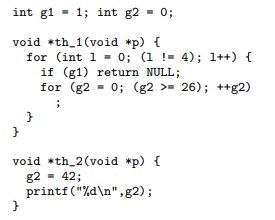
\includegraphics[scale=0.5]{EXAMPLE_COMPOPT_SRC.PNG}
            }
        \end{figure}

        The above code should print the value lf $g2$ to be $42$. 

        However, the above code when compiled using gcc 4.7.0 with -O2 enabled on x86-64 machine, the result of printf is $0$.  
        
    \end{frame}

    \note{
        The reason why it should be $42$ is that the value of $g2$ is never changed in $th\_1$.
        Notice that $g1$ has $1$, so the conditional will always return $NULL$.
        It is only $th\_2$ that writes to $g2$.
    }

    \begin{frame}{Behind the scenes}

        The above code is optimized using Loop invariant code motion in $th\_1$.
        However, the code that results due to it in x86-64 format is as below:
        \begin{figure}
            \makebox[\textwidth][c]{
                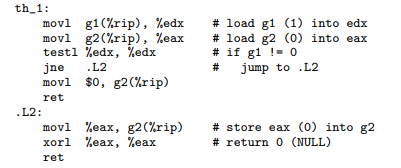
\includegraphics[scale=0.6]{EXAMPLE_COMPOPT_TRGT.PNG}
            }
        \end{figure}

        Notice the last $movl$ before return. 
        Here the value of $g2$ is restored to be $0$.
        This is sound if the program was sequential, however, in a concurrent setting this is clearly unsafe.
        
    \end{frame}

    \note{
        Here, the optimization tries to eliminate the inner loop.
        However, the process introduces some redundant writes, like that of $g2$ to be present.
        Thus, redundant write Introduction in this case becomes unsafe.
        This in turn makes such a variant of loop invariant code motion unsafe.  
    }

    \begin{frame}{Main idea of testing using traces: Another Example}
        Testing for such concurrency bugs is difficult. 
        For this purpose, we note that the concurrency bugs are only among those actions which involve a shared memory.
        So reducing the source program to a set of actions performed on shared memory can first be done. 
        This is followed by identifying the possible traces of these actions allowed by the program on its executions.
        The above code's problem can be observed by the following trace observed to be incorrect after optimization.
        \begin{figure}
            \makebox[\textwidth][c]{
                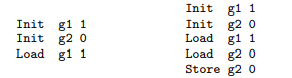
\includegraphics[scale=0.6]{EXAMPLE_COMPOPT_TRACE.PNG}
            }
        \end{figure} 

    \end{frame}

    \note{
        The memory model of C11 by this time was defined using traces / execution based semantics.
        It was more of utilizing this to do practical testing of C programs.
    }

    \begin{frame}{Overview of C11 memory model}
        
        To summarize the memory model, each shared memory access has a memory order. 
        Each action has an access, memory order and thread id. 
        \begin{figure}
            \makebox[\textwidth][c]{
                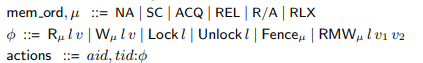
\includegraphics{C11MemoryModel.PNG}
            }
        \end{figure}

    \end{frame}

    \begin{frame}{Useful terminology used for optimization}

        \begin{itemize}
            \item Every concurrent program has various executions possible. 
            \item These executions involve various shared memory $actions$ that are done (even those due to multiple iterations of loop).
            \item A collection of these actions is defined to be an $opsem$. 
            \item $opsem$ also retains the syntactic order between actions belonging to same thread.
            \item All possible $opsems$ for a program is called $opsemset$. 
        \end{itemize}

        An example is as below;
        \begin{figure}
            \makebox[\textwidth][c]{
                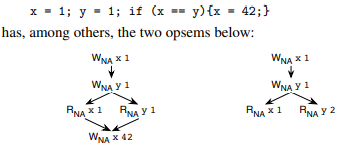
\includegraphics[scale=0.6]{OPSEM_EXAMPLE.PNG}
            }
        \end{figure}

    \end{frame}

    \begin{frame}{Effect of an optimization}
        
        \begin{itemize}
            \item The effect of an optimization is directly seen at the $opsem$ level. 
            \item For an $opsem$, an optimization has the effect of reordering, eliminating and introducing actions. 
        \end{itemize}

        The following example showcases this:
        \begin{figure}
            \makebox[\textwidth][c]{
                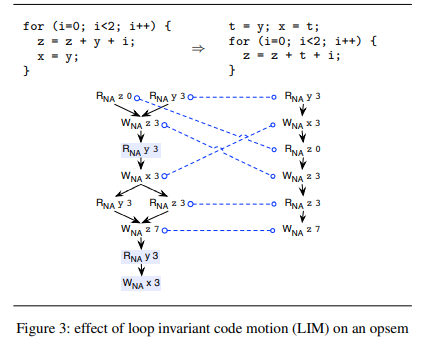
\includegraphics[scale=0.6]{OPSEM_EXAMPLE_LOOP_INV_CODE_MOTION.PNG}
            }
        \end{figure}

    \end{frame}

    \begin{frame}{Soundness of Optimisations}
        
        \begin{itemize}
            \item Every $opsem$ represents an execution.
            \item The outcome of the execution can be characterized as the final values in memory and the final read values.
            \item These two are represented together as an $obs$ or observable behavior. 
            \item A pair $opsem, obs$ represent a candidate execution.
            \item An optimization is sound if the set of $obs$ of the transformed program is a subset of that of the source program . 
        \end{itemize}
        
    \end{frame}

    \begin{frame}{Types of Optimizations considered}

        \begin{itemize}
            \item Elimination - eg: Read-after-Write, Write-after-Write, etc.
            \item Reordering - eg: Read-Write, Read-Read, etc.
            \item Introduction - Read / Write. 
        \end{itemize}
        
    \end{frame}

    \begin{frame}{Using above results for testing}

        Most bugs found in $gcc$ were that where writes were introduced in the program. 
        Some bugs were based on illegal reordering across atomic(SC) actions.
        The figure below showcases such a program 
        \begin{figure}
            \makebox[\textwidth][c]{
                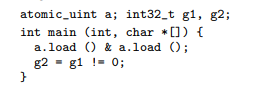
\includegraphics[scale=0.6]{TESTING_REORD_SRC.PNG}
            }
        \end{figure} 

    \end{frame}

    \begin{frame}{Trace analysis showcasing illegal reordering}

        $gcc$ test version disallowed any reorderings across atomic actions. 
        However, on trace analysis it was observed that the load of $g1$ was moved above the two atomic loads to $a$. 
        \begin{figure}
            \makebox[\textwidth][c]{
                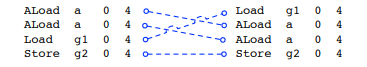
\includegraphics[scale=0.6]{TESTING_REORD_TRACE_INCORRECT.PNG}
            }
        \end{figure}

        Although in this case such a reordering does not result in any new outcome, introducing other concurrent threads running might result in some new behaviors.
        
    \end{frame}

    \note{
        The most simple example is that of message passing, where in this case $a$ is considered as an atomic flag variable and $g1$ as the message containing the data. 
        Reordering these two would result in a case where $g1$ has some data before the flag was set. 
    }

    \begin{frame}{Yet another interesting transformation}
        
        The following program gives us an interesting view of "bug" caused by transformation
        \begin{figure}
            \makebox[\textwidth][c]{
                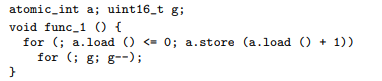
\includegraphics[scale=0.6]{TESTING_WEIRD_PROG.PNG}
            }
        \end{figure}

        On trace analysis, we note that a load to $g$ has been replaced by a store to $g$. 
        \begin{figure}
            \makebox[\textwidth][c]{
                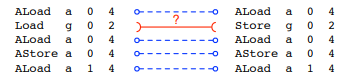
\includegraphics[scale=0.6]{TESTING_WEIRD_TRACE.PNG}
            }
        \end{figure}

    \end{frame}

    \begin{frame}{Is it a bug? }
        
        The above situation was caused by the following transformation
        \begin{figure}
            \makebox[\textwidth][c]{
                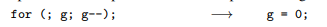
\includegraphics[scale=0.6]{TESTING_WEIRD_TRANSF.PNG}
            }
        \end{figure}

        The source program itself would not change the value of $g$, leaving it to be the deafult value $0$.
        In that sense, the transformation above does make sense, as a load is replaced by a redundant write to $0$.
        However, whether such a transformation should be allowed or not is a debate.
        Note that the introduced write could lead to cache contention where there shouldn't be any, leading to performance dipping down.

    \end{frame}

    \note{
        Its interesting that a transformation can in essence involve removing and inserting actions as an atomic step. 
        Definitely, the class of transformations one can do is infinte. :o
    }

    \begin{frame}{Thank you}

        Questions?

    \end{frame}


\end{document}